%%%%%%%%%%%%%%%%%%%%%%%%%%%%%%%%%%%%%%%%%%%%%%%%%%%%%%%%%%%%%%%%%%%%%
%																	%
%	CHAPTER TWO, HARDWARE IN HPV									%
%																	%
%%%%%%%%%%%%%%%%%%%%%%%%%%%%%%%%%%%%%%%%%%%%%%%%%%%%%%%%%%%%%%%%%%%%%

\chapter{Hardware in HPC}

\section{Introduction}

Optimization can't be done without a good knowledge of the architecture of the device, machine, or computer. 
Indeed, nowaday software and API try to take care of most of the cases but the last percent of gain have to be architecture dependent. 
In this chapter we will describe the most important devices architecures from classical Central Processing Units (CPUs), General Purpose Graphics Processing Units (GPGPUs), Field Programmable Gate Arrays (FPGAs) and Application-specific integrated circuits (ASICs).
Then those independants elements are use together in order to build supercomputers. 
The way they are arranged and the nodes interconnection is something that really matter at large scale.  

\section{Architectures}
\subsection{Classical CPU}

The CPU, as we know it today, begin its history with \textit{Texas Instruments Inc} and the first patent describing a CPU is "Computing systems cpu" proposed by \textit{Gary Boone} and published in 1973.
This first fonctional processing unit on chip and is based on the Von Neumann Model presented in chapter 1.
Before that vacuum tubes were used instead of transistors.



VECTORIZATIOONNNNN

\subsubsection{Intel}

We cannot decently present nowadays CPU without presenting the world leader that equiped around 90\% of the supercomputers (from November 2017 TOP500 list). 
Since 2007 Intel adopted a production model called the "Tick Tock", presented on Fig.~\ref{fig:1_HPC:intel_tick_tock}.

\begin{figure}
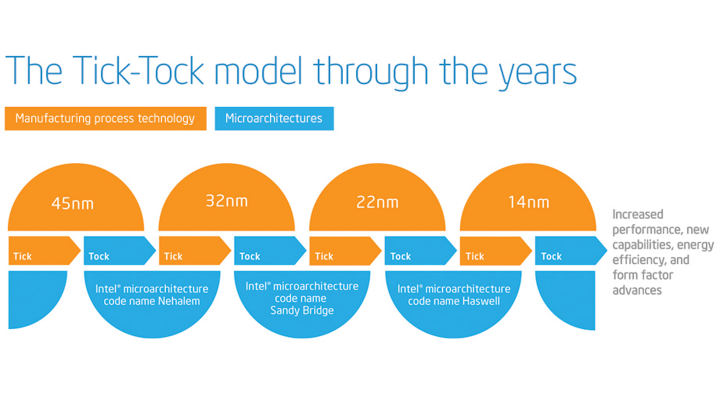
\includegraphics[width=\textwidth]{\locpath/figures/chap1/intel_tick_tock.png}
\caption{Intel Tick-Tock model}
\label{fig:1_HPC:intel_tick_tock}
\end{figure}

Since its creation the model was following the same fashion, a new manufacturing technology like shrink of the chip with better engraving on a Tick and a new microarchitecture delivered on a Tock

\subsubsection{ARM}
Advanced RISC Machines is a specific kind of CPU based on RISC architecture. 
Indeed, usual CPU implemented a complete Instruction Set Architecture, ISA, to perform complicated operations called CISC, Complex Instruction Set Computers. 
The downside is the complexity of CISC machines makes them hard to create and they use more energy. 
The ISA from the RISC is simplier and requires less transistors to operate. 
Therefore, the energy required and the heat dissipated is less important than for usual CPUs. 
It would then be easier to create massively parallel processors based on ARM. 

\subsection{GPGPU}

GPUs are based on the SIMD model of the Flynn taxonomy presented previously, \emph{Single Instruction, Multiple Data}.
The specific execution model is called SIMT (\emph{Single Instruction, Multiple Thread}). It enables the execution of millions of coordinated threads in a data-parallel mode. 
Two main companies provide GPGPUs for the HPC world NVIDIA and AMD, we will present them in that order and conclude on the differences. 

\subsubsection{NVIDIA GPU architecture}

The NVIDIA company was fonded in April 1993 in Santa Clara, Carolina, by three persons in which Jensen Huang, the actual CEO.
Its name seems to come from \textit{invidia} the latin word for Envy and vision, for the graphics generation. 

Known as the pioner in graphics, cryptocurrency, portable devices and now AI, it seems to be even the creator of the name "GPU".
It GPU, inspired from visualisation and gaming at a first glance, is available as a dedicated device  since the Tesla. 
The public GPUs can also be use for dedicated computation but does not feature eMMC memory, double precision or special functions/FFT cores. 

We will describe here the Kepler architecture, this is the one we worked

\begin{figure*}[t!]
\centering
\setlength\fboxsep{0pt}
\setlength\fboxrule{0.25pt}
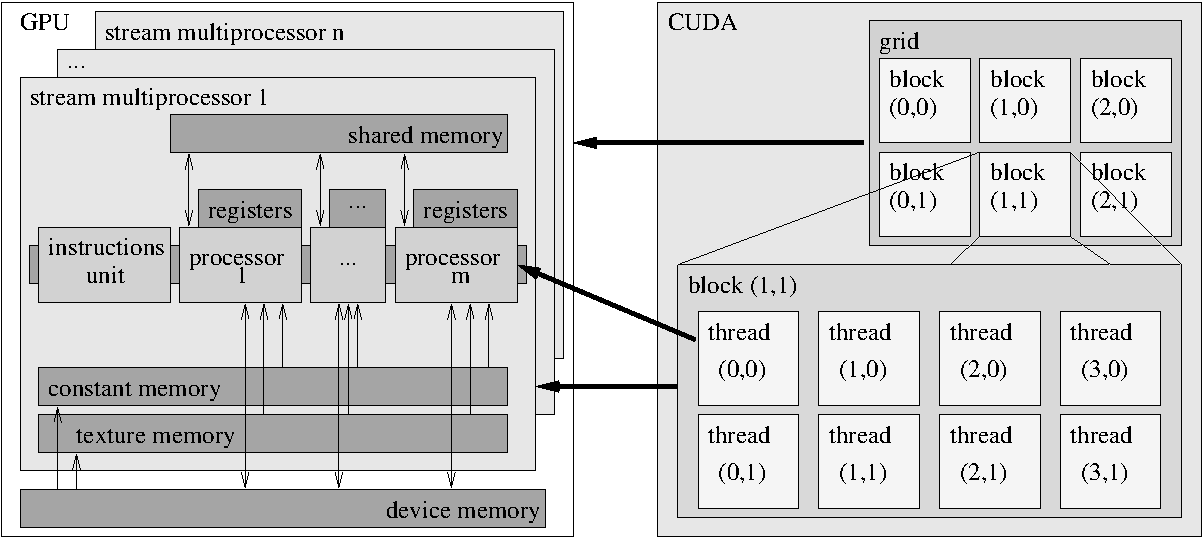
\includegraphics[scale=0.6]{\locpath/figures/chap1/smx}
\caption{NVIDIA GPU and CUDA architecture overview}
 \label{fig:chap1_gpu}
%\vspace{-0.8cm} 
\end{figure*}

As presented in Fig.\ref{fig:chap1_gpu}, NVIDIA GPUs include many \emph{Streaming Multiprocessors} (SM), each of which is composed of many \emph{Streaming Processors} (SP). In the Kepler architecture, the SM new generation is called SMX.
%
%In the CUDA programing model~\cite{cuda}, the GPU works as a SIMT co-processor of a conventional CPU. 
Grouped into \emph{blocks}, \textit{threads} execute \emph{kernel} functions synchronously.
Threads within a block can cooperate by sharing data on an SMX and synchronizing their execution to coordinate memory accesses; inside a block, the scheduler organizes \emph{warps} of 32 threads which execute the instructions simultaneously.
The blocks are distributed over the GPU SMXs to be executed independently.

\subsubsection{Memory, bandwidth and streams:}

In order to use data in a CUDA kernel, it has to be first created on the CPU, allocated on the GPU and then transferred from the CPU to the GPU; after the kernel execution, the results have to be transferred back from the GPU to the CPU. 
GPUs consist of several memory categories, organized hierarchically and differing by size, bandwidth and latency.   
On the one hand, the device's main memory is relatively large but has a slow access time due to a huge latency. 
On the other hand, each SMX has a small amount of shared memory and L1 cache, accessible by its SPs, with faster access, and registers organized as an SP-local memory. 
SMXs also have a constant memory cache and a texture memory cache.
%, that are linked to the constant and texture memories physically located in the device memory: these are read-only and have faster access time than the rest of the memory categories.
Reaching optimal computing efficiency requires considerable effort while programming.
Most of the global memory latency can then be hidden by the threads scheduler if there is enough computational effort to be executed while waiting for the global memory access to complete. Another way to hide this latency is to use streams to overlap kernel computation and memory load. 

\subsubsection{Threads synchronization:}
It is also important to note that branching instructions may break the threads synchronous execution inside a warp and thus affect the program efficiency. 
This is the reason why test-based applications, like combinatorial problems that are inherently irregular, are considered as bad candidates for GPU implementation. 
%This is particularly true with regard to combinatorial problems resolution. 
Thus we intend to provide a way to regularize their execution, in order to get good acceleration with GPU computation. 

\subsubsection{Details on K20Xm}

\todo{Describe K20Xm, 2688 cores}

\subsection{FPGA and ASICS}

\section{Interconnection and clusters}

\section{Interconnects}


\subsection{TOP500 remarquable clusters}
\subsubsection{Sunway Taihulight}

Sunway Taihulight is the third Chinese supercomputer to be ranked in the first position of the TOP500 list. \todo{(VERIFIER)}
A recent report from Jack Dongarra, a figure in HPC, decrypt the architecture of this supercomputer\cite{dongarra2016report}. 
The most interessant point is the conception of this machine, completely done in China. 
The Sunway CPUs were invented and built in China, the Vendor is the Shanghai High Performance IC Design Center. 

\begin{figure}
\centering
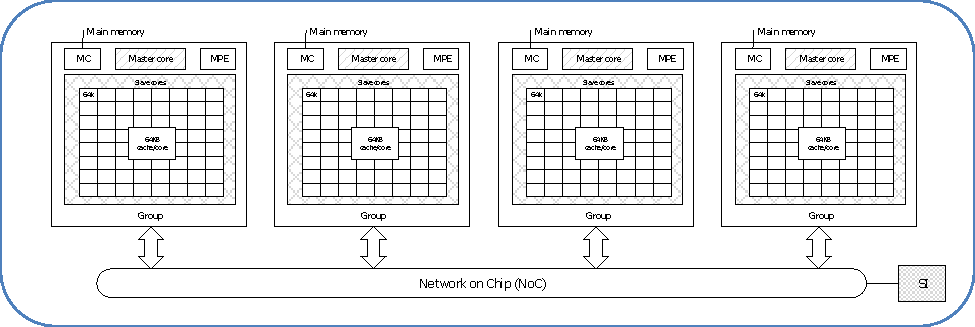
\includegraphics[scale=1]{\locpath/figures/Chap1/report_sunway_CPE}
\caption{Sunway Taihulight node architecture from \textit{Report on the Sunway TaihuLight System}, Jack Dongarra, June 24, 2016.}
\label{fig:chap1_report_sunway_CPE}
\end{figure}

The SW26010, a many core architecture, features 260 cores based on RISC architecture and a specific conception depicted on Fig.\ref{fig:chap1_report_sunway_CPE}.


\subsubsection{Titan}

\subsubsection{K-Computer}
\subsubsection{Sequoia}
\section{ROMEO Supercomputer}

The ROMEO supercomputer center is the computation center of the Champagne-Ardenne region in France. 
Hosted since 2002 by the University of Reims Champagne-Ardenne, this so called meso-center (French name for software and hardware architectures) is used for HPC for theoric research and domain science like applied mathematics, physics, biophysics and chemistry. 

This project is support by the Champagne-Ardenne region and the CEA (French Alternative Energies and Atomic Energy Commission), aim to host research and production codes of the region for industrial, research and academics purposes. 

We are currently working on the third version of ROMEO, installed in 2013. 
As many of our tests in this study have been done on this machine, we will carefully describe its architecture. 

This supercomputer was ranked 151st in the TOP500 and 5th in the GREEN500 list. 

\subsection{ROMEO hardware architecture}
ROMEO is a Bull/Atos supercomputer composed of 130 BullX R421 computing nodes. 

Each node is composed of two processors Intel Ivy Bridge 8 coeurs @ 2,6 GHz. 
Each processor have access to 16GB of memory for a total of 32GB per node, the total memory if 4.160TB. 
Each processor if linked, using PCIe-v3, to an NVIDIA Tesla K20Xm GPGPU. 
This cluster provide then 260 processors for a total of 2080 CPU cores and 260 GPGPU providing 698880 GPU cores. 
The computation nodes are interconnected with an Infiniband QDR non-blocking network structured as a FatTree. 
The Infiniband is a QDR providing 10GB/s. 

The storage for users is 57 TB and the cluster also provide 195 GB of Lustre and 88TB of parallel scratch filesystem. 

In addition to the 130 computations nodes, the cluster provides a visualization node NVIDIA GRID with two K2 cards and 250GB of DDR3 RAM. 
The old machine, renamed Clovis, is always available but does not features GPUs. 

The supercomputer supports MPI with GPU Aware and GPUDirect. 
